\chapter[Spatial proteomics for mapping cell types and identifying interactions across tissues]{Spatial proteomics for mapping cell types and identifying interactions across tissues}
\label{Chap:3}	%CREATE YOUR OWN LABEL.
\pagestyle{headings}
\section{Introduction}
\label{Sec:3.1_intro}
%CREATE YOUR OWN LABEL.
Recently, there has been a dramatic growth in the number and type of cell surface proteins that can be profiled in experiments, enabling the identification and validation of predictive biomarkers easier than ever. In fact, many highly multiplexed IHC platforms have been approved by FDA (Food and Drug Administration) to be used in clinical routine \cite{van2021multiplexed, hawes2009immunohistochemistry,decalf2019new}. As discussed in Chapter \ref{Chap:Intro}, there are two main approaches to spatial proteomics including multiplexed fluorescence and mass spectrometry imaging technologies. The analysis results in this chapter are from using input data of both experimental approaches. Specifically, I applied the spatial cellular analysis to specimens of human skin cancer and colorectal cancer with Opal Polaris 6-plex PD1-PDL1 panel and 16-plex Hyperion Imaging Mass Cytometry (IMC), respectively.        

In the first project, Opal IHC Polaris spatial proteomic data of six whole slide tissue samples from 3 patients with SCC/BCC was generated. The Polaris PD1-PDL1 panel for skin cancer consists of six proteins including CD8, PD-L1, PD-1, FoxP3, CD68, Pan-cytokeratin (PanCK), and DAPI for nuclei staining. In non-cancer cells, PD-1 is known as the immune checkpoint inhibitor that binds to immune cell PD-L1 ligand to keep T cells from over-activating and attacking normal cells in the body. Some cancer cells, particularly epithelial-derived cancer cells, can exploit the mechanism to suppress immune responses to induce tumorigenesis \cite{tsai2014pd, chen2013oncology}. Therefore, the first part of this chapter will use the pair of proteins PD-L1 and PD1 as the case study to investigate cell type colocalisation and co-occurrence in skin cancer (Figure \ref{fig:Polaris_skin_cancer_preprocessin}A). Additionally, we leverage the analysis to detect cell communities within skin cancer samples in the context of cancer-immune infiltration.  

In the second part, we focus on colon adenocarcinoma (COAD), the most common type of colorectal cancer which is also ranked as the third most common cancer type \cite{wang2022identification, siegel2021cancer}. Although the immunotherapy treatment for COAD has greatly improved, often many patients (more than 50\%) do not respond to treatment. The second part analyses the interaction between cancer and immune cells from low-order to high-order spatial signatures using data generated from the Hyperion IMC platform \cite{giesen2014IMC}. Unlike Polaris technology, IMC performs tissue scanning at multiple regions of interest (ROIs) selected from whole slide tissue. The experiment was designed to capture the panel of 16 protein markers from 51 patients with stage 3 colon adenocarcinoma. A total of 170 ROIs were measured. The IMC protein panel consists of structural protein markers specific for Epithelial cells (E-cadherin, Keratin), Fibroblast (Collagen), proliferative epithelial (Ki-67 positive), and several immune markers including for T-cells (CD8), regulatory T cells (FoxP3), macrophages (CD68+), and B cells (CD20+).  Although the two input datasets captured different antibody panels as well as different cancer types, they both produce protein profiles at subcellular resolution retaining a wealth of spatial information.    

We reasoned that the interactions between cell types within the tissue are beyond the cellular level, happening at a higher-order scale. Cells within the tissue are organised into multiple compartments and structures with distinct functions. By analogy, different cell types in the spatial context are considered individuals with different jobs (i.e. teachers or doctors) in human society. At a higher granular level, the tissue communities are equivalent to facilities (i.e. industrial, hospitals) that are specialised in functions. Therefore, identifying the interaction at the different granularity and integrating information between them allows us to better understand the tissue's behaviour \cite{schurch2020coordinated}. Advances in experiment technologies and computational methods have allowed the association analysis between the tissue spatial communities and clinical outcome or genomic alteration \cite{schurch2020coordinated, danenberg2022breast}. For this chapter \ref{Chap:3}, I focused on high-order of spatial organisation and the cross-talk between cell types in cancer tissues.

The implementation of several of our analyses leveraged some existing functions from squidpy \cite{palla2022squidpy} and histocat \cite{schapiro2017histocat} to facilitate the adaptation to tissue landscapes in our dataset. Regarding the co-occurrence analysis from squidpy, the default function assumed that the input data is captured by ROIs. The assumption has a disadvantage that prevents the co-occurrence scores to converge in a free-form input (i.e. elongated ROI or tissue). As the Opal Polaris imaging data captured the whole slide tissue, we customised the function to limit the observation radius to a flexible threshold. The flexible threshold can warranty the co-occurrence scores to converge. Besides, we also tested the co-occurrence scores from multiple ROIs to find the significant pair of interaction cell types. Additional detail about the improvements will be specified in the sections \ref{Sec:3.2_SP_celltype_id_pipeline}.

\begin{table}[ht]
\centering
\caption{Summary of data specification}
\begin{tabular}{||P{7cm} || P{3cm} || P{3cm} ||} 
 \hline
 Specifications & Colorectal Cancer Samples & Skin Cancer Samples   \\ [0.33ex] 
 \hline\hline
 Number of patients & 52 & 3   \\ 
 \hline
 Number of Markers & 16 markers & 6 markers  \\ 
 \hline
 Number of images & 126 ROIs &  6 whole slides \\
 \hline
 Diagnosis & Stage 3 adenocarcinoma & Basal Cell Carcinoma  \\ [1ex] 
 \hline
\end{tabular}
\label{table:DataInfor}
\end{table}
% ***************************************************
\section{Cell type identification and cell communities detection methods}
\label{Sec:3.2_SP_celltype_id_pipeline}	%CREATE YOUR OWN LABEL.
\subsection{A pipeline for cell type identification from spatial proteomic data}
Highly multiplex IHC  or IMC often represent the spatial proteomic data as multi-channel images. Therefore, image processing in the form of single-cell segmentation is often required as a data preprocessing step. Single-cell protein expression values were measured as the mean intensity of ion count from antibodies labeled by heavy metals or fluorescent signal encompassed within the cell mask (i.e. cell border defined from segmentation). Considering fluorescent signal intensity or ion count as a measurement for protein expression can create some technical challenges, for example how the data can be normalised when combining the data from multiple ROIs or tissues. Therefore, we also introduced several signal-gating and data filtering to each dataset accordingly to facilitate cross samples normalization and integration. Specifications about the single-cell data processing for each datatype will be detailed in this section.  

For the first project, each skin cancer sample contained around $40000\sim 79000$ cells per tissue, depending on the size of the whole slide tissue section. To employ the currently established cell clustering and annotation, the Opal Polaris imaging was transformed into a non-imaging-based data through cell segmentation process (Figure: \ref{fig:Polaris_skin_cancer_preprocessing}A-B) \cite{hickey2021strategies}. More specifically, cell segmentation was carried out throughout the tissue using a deep learning model called StarDist \cite{schmidt2018cell}, which eventually turned every nuclei in the DAPI channel into a list of cell objects. For each cell object, the protein signal intensity was normalised to the mean DAPI intensity within the cell boundary and assigned to the expression level of that protein to the cell (Figure: \ref{fig:Polaris_skin_cancer_preprocessing}B-D). To remove the noisy high background from fluorescent intensities (outliers), we added a custom threshold of $95^{th}$ percentile which was used to cap the maximum value of each marker (Figure: \ref{fig:Polaris_skin_cancer_preprocessing}D-E). After the preprocessing step of imaging data, a standard cell-type clustering was applied using a common single-cell processing pipeline, scanpy \cite{wolf2018scanpy}. Based on the panel of 6 proteins, we were able to identify several major cell types, including epithelial cells (PanCK+), inmate immune cells (CD68+), and adaptive immune cells (CD8+, FoxP3+) (Fig: \ref{fig:skin_cancer_polaris}A). Among all the clusters detected by the scanpy Leiden clustering, those cells with very low expression of all the proteins in the panel were classified as unidentified and removed from downstream analysis. The cell identifications were eventually plotted back to the original spatial context for validation.  

Similarly, for our IMC imaging dataset of colorectal cancer, the starting analysis steps are cell segmentation and cell clustering. The key differences between Polaris and IMC are the resolution of the images generated by each technology. While every pixel in the Polaris image captures $0.49 \mu m$ in the real tissue, the specification in IMC is $1$pixel representing $1\mu m$. IMC generated discrete ion count signals (counts of heavy metal molecules from labeled antibodies) which required a specialised cell segmentation method. Currently, the IMC segmentation pipeline is being adapted from a pipeline by Bodenmiller Group, one of the founders of the technology (\href{https://github.com/BodenmillerGroup/ImcSegmentationPipeline/blob/development/scripts/imc_preprocessing.ipynb}{Github IMC preprocessing pipeline}. Using the existing data preprocessing tool, the raw IMC data (.mcd file) is converted into a standard image format with multiple channels (OME tiffs) and each channel represents the expression of a protein staining marker (Figure: \ref{Chap3:fig:IMC_cell_type_annotation}A). 

Because the signal intensity in IMC has a lower resolution yet is noisier than in Polaris, we manually built a segmentation model to assign pixels to either cell nuclei, cytoplasm, or background. In collaboration with a team member, who has a clinical background, we assigned  the pixel annotation to a subset of cells in the whole ROI using CellProfiler and Ilastik \cite{carpenter2006cellprofiler, berg2019ilastik}. The trained pixel classification model from Ilastik was performed across the whole dataset to segment the cells from the background. Since IMC imaging data was generated only for selected ROIs, the number of cells in this project is significantly lower than that in the skin cancer project, ranging from $200$ to $1600$ cells per ROI (approximately 2-3 ROIs per sample). After the cell segmentation, customised single-cell data preprocessing is applied to map signals to a list of cell objects. Cellular data was also clipped to remove outliers. Additionally, cells that were either too small (due to  signal noise) or too large (possibly overlapped cells) were filtered from the downstream analysis. By applying the harmony algorithm for single-cell data from multiple rounds of experiments, a total of 903,125 cells were merged for further analysis. For cell type annotation, major structural cell types were identified with high confidence such as Epithelial/Cancer (E-cadherin and Keratin), Proliferative Tumour (KI67+), and Stromal (Collagen, SM-actin). We were also able to annotate other adaptive like B-cells (CD20), cytotoxic T-cells (CD8+), Lymphocytes (CD4+), Natural Killer cells (FoxP3+), and Macrophages (CD68) (Fig:\ref{fig:colorectal_cancer_IMC}A). For validation, we compared the IMC-identified cell types against pathologist annotation. Through a process called image registration, we were able to align the IMC image to the adjacent section of H\&E image which was annotated with some cell types by the pathologist (Fig:\ref{fig:colorectal_cancer_IMC}B). Since our computational results matched well with manual annotation this gave us confidence in our cell segmentation and clustering approaches before proceeding to the CCC analyses. 

\begin{figure}[htp]
    \centering
    \includegraphics[width=\columnwidth]{Chapter3/Figures/Chap3_Figure1_1.png}
    \caption[Schematic of spatial data preprocessing for cell type annotation.]{ Opal Polaris spatial data preprocessing for cell type annotation. (A) Polaris spatial proteomic data from the SCC patient B18 with the pathological annotation, based on tissue morphology. (B) A zoomed-in image of cell the nuclei representation in DAPI channel (dark blue) and cytokeratin marker expression (PanCK in red) for epithelial cell marker. The annotation line in white colour separates the cancer lesions of the skin from the lower layer. (C) Detection and segmentation of cells from the image using the nuclei channel. (D) The conversion of imaging-based data to single-cell-based data by measuring the level signal each cell expresses within the cell boundary. (E) Histograms of the expression level of each protein in the panels across all the detection cells}
    \label{fig:Polaris_skin_cancer_preprocessing}
\end{figure}

\begin{figure}[htp]
    \centering
    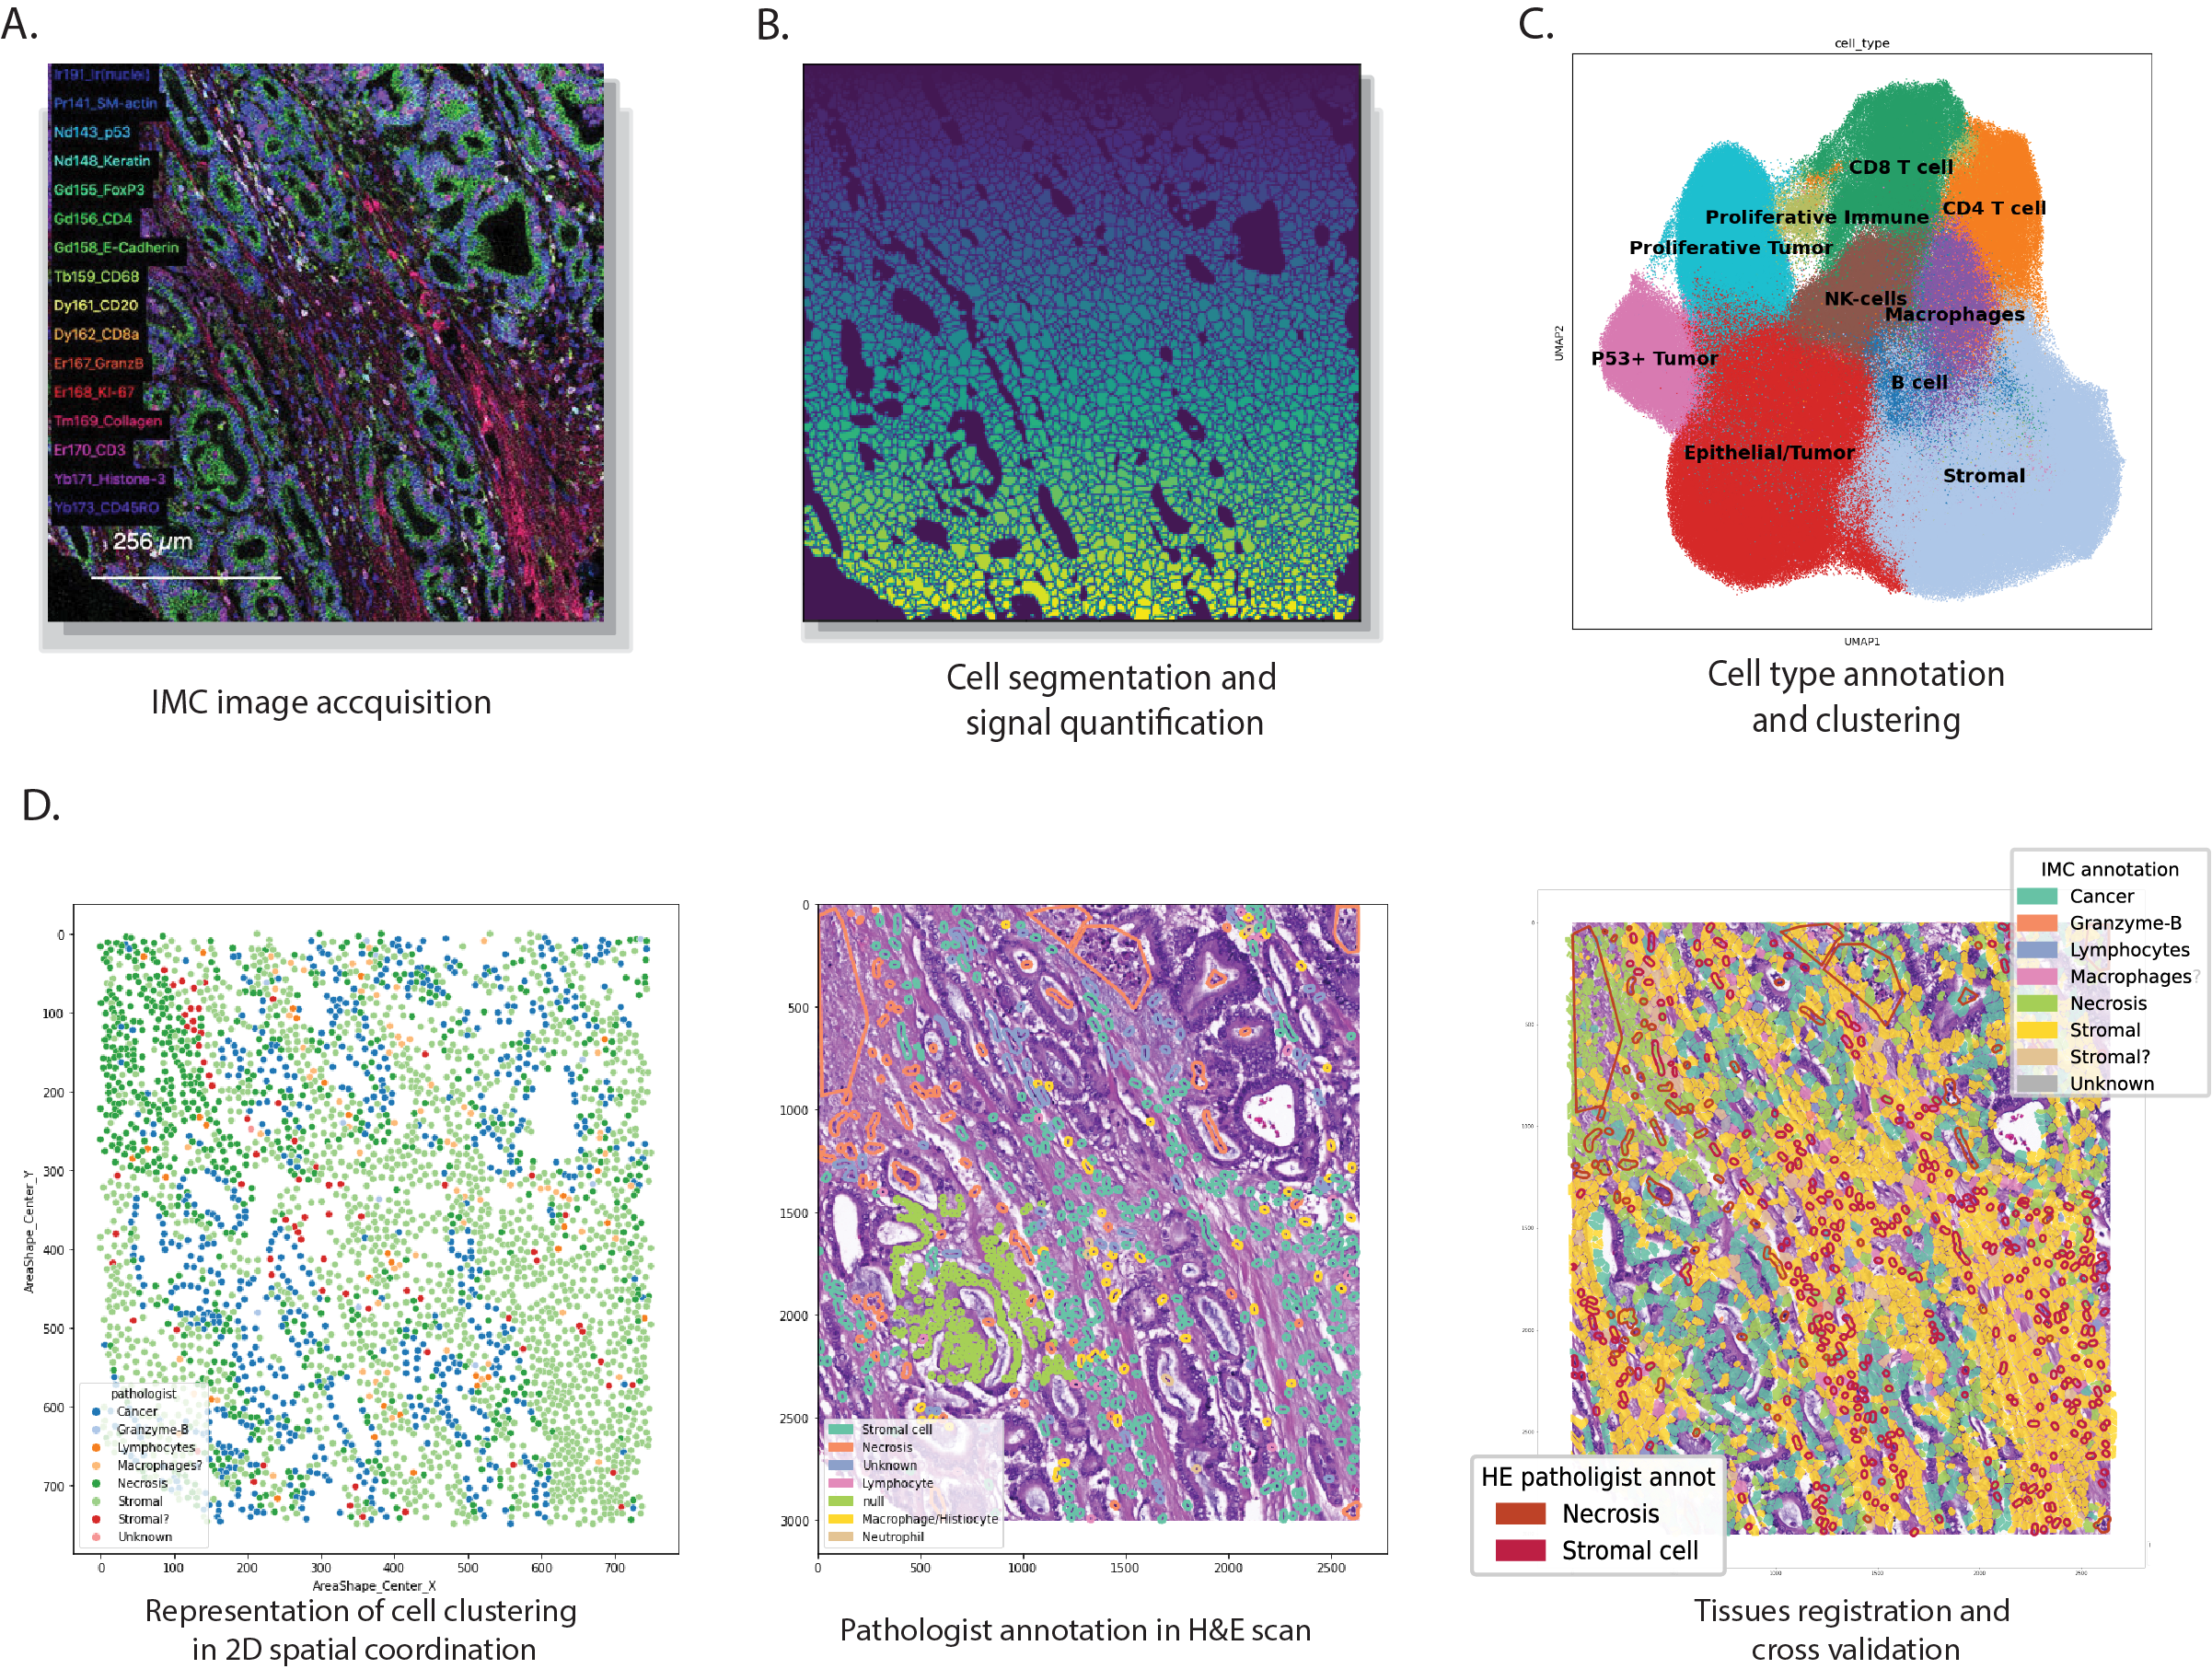
\includegraphics[width=\columnwidth]{Chapter3/Figures/Chap3_Figure2_IMC_CellID.png}
    \caption[Hyperion Imaging Mass Cytometry cell identification process]{The workflow for the transformation IMC data from multiplexed imaging data to single-cell proteomic matrix (A) The standard mcd files from Hyperion IMC platform were converted into multiple channel OME-tiff file. Each channel of a tiff image represents a protein staining channel. (B) A pixel classification model was manually generated specifically for the whole dataset to perform cell segmentation. (C) Cells from multiple ROIs were merged, clustered, and annotated. (D) Annotated cells could be plotted back to the original spatial context for validation using pathologist annotations.}
    \label{Chap3:fig:IMC_cell_type_annotation}
\end{figure}
\subsection{Detecting cell communities using spatial distribution}
\label{Sec:3_cell_communities_and_coocurrence}	%CREATE YOUR OWN LABEL.
To capture the high-order higher-order scale of spatial features, we performed cell communities detection. More specifically, we perform a clustering analysis to group the cells from the same neighbourhood with similar local densities of cell types. For each cell across the tissue, we identified the neighbouring cells using $10$ nearest neighbours within a radius of 100$\mu$m from the query cell. The neighbouring profiles of every cell across the tissue were aggregated and clustered using K Means. Quantitative measurement of cell composition for each community can provide insight into the biological interpretation of these communities.  

% \subsection{Applying nearest neighbourhood approaches to cell-cell interaction}
% ********* Enter your text below this line: ********
For the Polaris skin cancer dataset, we investigated how different cell types are colocalised into communities. Using the cell communities detection method, we identified five cell communities distributed across the tissue. Quantitative assessment of cell composition in each community allowed us to deduce biologically interpretable features of these communities (Fig: \ref{fig:skin_cancer_polaris}A). Particularly, communities 2 and 3 consisted of scattered immune cells while community 1 appeared to have a very high density of epithelial cells positive with PD-L1. This could be explained by the known biological process and tissue structure that cancerous epithelial cells tend to reside densely around the cancer nest, and the presence of immune cells under the epidermis layer (Fig: \ref{fig:skin_cancer_polaris}B, E). On the other hand, clusters 1 and 4 contain mixed epithelial and immune cell populations in the same communities. Comparing the distribution of cell communities and tissue annotation (Fig: \ref{fig:skin_cancer_polaris}B) suggested that the clusters 2, 3 and 4 highly aligned with the stromal microenvironment communities (Fig: \ref{fig:skin_cancer_polaris}D).  Of note, using our own STRISH test (described in more detail later), we found spatially-specific interactions between PD1 and PDL1 along the edge of cancer and immune cells \ref{fig:skin_cancer_polaris}C). 

Given the cell communities detection result, we further investigated how the cell clusters 2 and 3 (immune communities) by co-occurrence analysis (Fig: \ref{fig:skin_cancer_polaris}E, F). As mentioned before, the co-occurrence score is measured by the fraction of the probability of observing a condition cell type in the presence of a reference cell type over the probability of the observing condition cell type co-occurs with any random cell type. After that, K-function was used to summarise the co-occurrence of specific cell types with all other cell types across increasing distance intervals. Note that because the skin biopsies are wide but narrow, the cell type co-occurrence scores are expected to diverge after converging. We customised the function to measure the co-occurrence score using 50 $\mu$m interval within the range from 0$\mu$m to 600$\mu$m (95\% of the pairwise distance between condition cell type and others). Using CD8 T-cells positive with PD1+ protein as the condition (reference) cell type), the co-occurence test confirmed that the co-localisation of these cells with the other two subgroups of T-cells, including double positives CD8+ and FoxP3+ and single positive CD8+ T-cells were higher than random (at distances from $0\mu m$ to $400 \mu m$). Similarly, PanCK+ was also found to be co-occurred with the CD68+ and PD1+ double-positive clusters, consistent with the result from our community detection analysis \ref{fig:Polaris_skin_cancer_preprocessing}.     

Applying similar CCC analysis approaches to the colorectal dataset, we sought to test for the co-localization between cancer and immune cells across ROIs. As an example, the general distribution of cells and signals within an ROI is shown in \ref{fig:colorectal_cancer_IMC}A and \ref{fig:colorectal_cancer_IMC}B. Figure \ref{fig:colorectal_cancer_IMC}D shows the probability of observing a cell type conditioned on the presence of cancer cells of the ROIs showed in \ref{fig:colorectal_cancer_IMC}A. We could observe a high enrichment of cancer cells with epithelial cells at the first $200\mu m$ interval. While the co-occurrence analysis could provide insights into how different cell types form cell communities, the analysis is limited to a single ROI at a time. Therefore, we performed an additional analysis where we grouped co-occurrence scores of multiple ROIs together which allowed us to statistically test (Wilcoxon test) for the significance of co-localization relative to the population average. The table embedded in the Figure\ref{fig:colorectal_cancer_IMC}E shows the significant test of occurrence scores between every pair of cell types in our dataset. This new statistical test framework is being developed, and the preliminary results suggested differential cell type co-localisation across patients and should be suitable features to be correlated with clinical outcomes.

\begin{figure}
    \centering
    \includegraphics[width=0.8\columnwidth]{Chapter3/Figures/Minh_figure3-01.png}
    \caption[Analyses of Polaris multiplexed imaging of human SCC skin cancer tissue. ]{High-order analyses of Polaris multiplexed imaging data of human SCC skin cancer tissue. (A) Cell type classification through clustering and signal gating of the expression of 6 proteins mapped to single cells. The panel of 6 antibodies was used to profile the protein expression of major interest cell types, including cytokeratin, cancer cells secreting immune inhibitor (PD-L1), and immune cells (CD8 T-cell, NK cells, Macrophages). (B) Pathological annotation of cancer and immune regions, based on tissue morphology. (C) Analysis of cancer-immune cell co-localisation through the ligand-receptor pair PD1 and PD-L1. (D) Voronoi map using the spatial distribution of the cell communities to split the original tissue into multiple regions, representation of distinct cell neighbourhood communities defined via clustering}
    \label{fig:skin_cancer_polaris}
    
\end{figure}
\subsection{Implementing and developing a contact-based approach for CCC analysis}
For the colorectal cancer project, we do not have the pathologist annotations for all the ROIs. Therefore, we adopted a slightly different approach to measure near-distant CCC. Using the cell segmentation masks as the representation of the cells, we expanded the peripheral of the cell by a margin of 6 pixels and counted the number of cells in direct contact within the adjacent space for pairwise interaction analysis (Figure: \ref{fig:colorectal_cancer_IMC}C). The pairwise interaction was compared to a random distribution using two individual one-tail permutation tests within the same image. These two one-tailed permutation tests produced two $P_{values}$ indicating the direction of communication between every pair of cell types, either interaction or depletion. The test suggests how significant a pairwise interaction between two cell types was compared to random, and eventually suggests an interaction or an avoidance trend. The significance ($P<0.05$) of the contact-based neighbourhood analysis in one of the ROIs shows the most significant interaction starting from epithelial cells toward fibroblast cells. The next significant interactions included those of cancer cells with macrophages and with NK-cells (equally) (Fig: \ref{fig:colorectal_cancer_IMC}D). These results make biological sense and are expected as the cause of colorectal adenocarcinoma are mutated epithelial cells which trigger the growth of surrounding stromal cells \cite{bremnes2011role}. 

% histocat approach which uses the cell outline
\begin{figure}
    \centering
    \includegraphics[width=0.8\columnwidth]{Chapter3/Figures/Chap3_figure4.png}
    \caption[High-order cell spatial  analysis result of IMC data.]{High-order cell spatial  analysis result of IMC data (A, B) The cell type and the Voronoi diagram of cell communities detection results of the patient id CR020 (C) The pairwise cell-cell interaction through the contact-based approach. (D) The co-occurrence analysis of different cell types in the presence of cancer cells at increasing distance threshold (E) A summary of significance co-occurrence score across all combinations of observed and expected cell types.}
    \label{fig:colorectal_cancer_IMC}
    
\end{figure}
% ***************************************************
\section{Developing STRISH for cell co-localisation with spatial proteomic data}
\label{Sec:3.Cell_colocalisation_PD1_PDL1}	%CREATE YOUR OWN LABEL.
Spatial information at the subcellular level can facilitate a lower level of spatial analysis, which uses the cell geometry and density to assist the interaction analysis. As described before, in the Polaris dataset, we scanned all the regions, where cancer and immune cells co-localised and interacted via PD-L1 and PD1. Using the cell clustering information, I developed and applied a STRISH scanning window strategy to search for regions where there are immune cells double positive for CD8+ and PD1+ in the immediate vicinity of cancerous epithelial cells (which themselves are double positive for PanCK+ and PD-L1+). The STRISH scanning window strategy starts with a broad scale (i.e 4 non-overlapped tiles at the size of of one fourth of the original slide scan) and gradually splits large tiles into smaller windows until a cell-count threshold is met (less than 100 cells per window by default). Subsequently, the results from cell detection are scored, normalised, and used to plot a heatmap for localised regions (neighbourhood) with co-localisation of the two cell types being tested. Figure \ref{fig:skin_cancer_polaris}C shows the activity map of CD8+, PD1+ cells, and PanCK+, PD-L1+ cells throughout the tissue. Interestingly, these two cell types were mostly observed to be co-localised at the interface of cancer and immune infiltration, according to the pathologist's annotation. The heatmap provided visual and quantitative evidence of CCC occurring between cells in our tissue sample. This analysis result is being integrated into a multimodal project to create an atlas of skin cancer and cell-cell interaction with other 5 complementary technologies (the manuscript is being under review).

Regardless of the input datatype, all the multiplexed imaging technologies, which capture gene or protein expression at the subcellular level, can be processed by a similar workflow. Collectively, the data processing should include data transformation into a standard multidimensional image data, cell segmentation, and signal mapping for each staining channel \cite{shakya2020immune, liu2019comparison, aghaeepour2013critical}. In this thesis, I first developed a pipeline for RNAscope data and then extended it to various types of spatial omic data. After the first version, some major refactoring to the STRISH pipeline were made to turn this pipeline to a more versatile framework. 

As mentioned above, after standard data preprocessing, the resulting multidimensional image is converted into a single-cell data matrix. A set of new functions for data loading to STRISH are added so that STRISH object can interact with an Anndata object \cite{wolf2018scanpy} to take advantage of this data object structure commonly used for single-cell matrices. Additional spatial coordination information is included in the object. This approach allows us to customise the object while still making use of various methods of single cell data normalisation and clustering methods. 

For CCC analysis, STRISH introduces a new method for cell co-localisation detection through windows scanning. STRISH identifies whether there are cells that express compatible ligands and receptors that locate within the tissue window (local microenvironment) and summarises the results in an interpretable heatmap. As the tissue fluorescence image contains gaps between cells, this makes tissue segmentation a challenging task. In STRISH, it is possible to use the scanning windows to accommodate for these gaps for calculating co-localisation. STRISH generates tissue contour to highlight the tissue region from the background. Several recent analysis features include automated cell segmentation and cell type clustering integrated with spatial information; nearest neighbourhood and co-occurrence approaches are also included in the framework. Finally, to increase the adaptability of multimodal analysis, image registration to align two tissue images from different rounds of experiments with minor variations is also included.   

It is important to acknowledge that STRISH particularly focuses on CCC analyses in spatial transcriptomic and proteomic data. Hence, it should not be used in isolation but in combination with other data normalisation and cell type clustering tools. Existing tools such as Giotto and Squidpy also provide multiple functions for spatial analysis and interactive graphical user interface. While such features are useful for exploratory analysis, STRISH features are tailored to cell-cell interaction through ligand-receptor and multimodal data analysis. 

% To improve STRISH, I also seek to introduce more statistical tests and spatial quantitative measurement into the current pipeline.
\section{Discussion}
Knowing that the relationship of cancer-immune interaction in cancer and the heterogeneity of cancer is a bi-directional incident. In this chapter, we presented multiple spatial analysis results to identify cell communities and how the cells communicate through distance. As the spatial proteomic platforms perform tissue imaging differently, we addressed some limitations of conversing the imaging data to single-cell data and introduced the data quality control for data preprocessing. Additionally, we demonstrated the power of performing multiple spatial analyses to validate the findings of each other. That allows us to deduce the biological interpretation of the analyses.      

For the second project of IMC for colorectal cancer, a statistical test to combine the multiple ROIs and tissue sample together for survival prediction and clinical outcome using CCC is also another analysis that I will implement and present in Chapter \ref{Chap:4}. The next goal of this thesis is to develop a holistic framework to work with multimodal spatial -omic data and discover different characteristics of CCC throughout cancer tissues and across patients. 

% \section{Quantitative and qualitative measurements}
% \label{Sec:3.4_validation}	%CREATE YOUR OWN LABEL.

% \subsection{Quantification of cell communities conserved across patient groups}
% % ********* Enter your text below this line: ********
% We introduce 
% \subsection{Comparison of tissue heterogeneity across patients and cancer subtypes}
% % ********* Enter your text below this line: ********
% By aggregating cell's neighbourhood from multiple ROIs, STRISH allows the spatial differential analysis across the  conditions and uncover the relationship between treatment outcome and spatial organisation of cell types.

\section{Appendix}
\begin{figure}[htp]
\renewcommand{\figurename}{Supplementary Figure}
    \centering
    \includegraphics[width=0.75\columnwidth]{Chapter3/Figures/Chap3_supple_figure_1.png}
    \caption[Analyses results of Polaris across multiple SCC and BCC samples]{Analyses results of Polaris across multiple SCC and BCC samples. (A,B) From top to bottom are the cell type identification, pathologist annotation, the heatmap of cell colocalisation through the pair of PD1-PDL1, and the cell type composition for each cell type community detected across the tissue sample from the patient ID R01 with SCC. (C) The equivalent analysis results for the tissue samples from the patient ID P04 with BCC}
    \label{fig:Chap2_Supfigure7}
\end{figure}
% ***************************************************
% \bibliographystyle{elsarticle-num}

% \bibliography{./References/Bibliography}

% There are already a few computational methods that used scRNA-seq to infer the CCC i.e. CellChat \cite{jin2021CellChat}, CellPhoneDB \cite{efremova2020cellphonedb} or NicheNet \cite{browaeys2020nichenet}. However, they are all unable to address the spatial constraints of interactions. With scRNA-seq data, the limited insights into the spatial location of the RNA molecules within a cell and the organization of cells in a tissue prevent the CCC inference from reaching its potential. To address this, the development of higher multiplexed histological techniques for capturing transcriptomic or/and proteomic information at subcellular resolution, e.g. co-detection by imaging (CODEX) \cite{goltsev2018CODEX} or IMC from Hyperion, facilitated the integration of spatial information into CCC inference. 

% Despite the rapidly growing number of spatially resolved transcriptomic and proteomic technologies, the currently available analysis strategies to process these high dimensional data have not yet exploited the full potential of spatial information. In short, spatially resolved CCC analysis can be categorised into two main categories. The first approach considers each cell as a point in Cartesian coordinate system and assesses the changes in the spatial co-localisation between pairs of cell types at distances \cite{arnol2019modeling,schurch2020coordinated}. Meanwhile, the second category considers the interactions of individual cells and their intermediate adjacent cells within a short proximity from the cell membrane. It is sufficient to measure cell-cell interaction through gap junction or paracrine signalling. The pairwise interaction of two cell types is then grouped by cell phenotypes and compared to randomised labels of cells to determine the significance of interactions  \cite{schapiro2017histocat}. In the following sections, I will go deeper into the advantages and disadvantages of each approach and how I applied them throughout my second-year projects.    

% PD1 has been extensively studied and identified as immune inhibitor for skin cancer cell growth\cite{ishida1992induced,  tsai2014pd}. In the first project using skin cancer as the model to study, we were interested in finding and validating the immune-cancer cell interactions pairing the ligand-receptor PD-L1 and PD1 through a series of spatial analysis methods. On the other hand, we sought to find the pattern of intercellular architecture in colorectal cancer and the correlation between alterations in CCC and the prognosis for the patients. Once the cells were clustered and annotated appropriately, we to applied multiple spatial analyses to study cell-cell interactions with the aim of improving the capability to predict the clinical outcome. For each project, we performed two to three neighbourhood analyses to explore and quantify the tissue section finds.  